\documentclass{article}

\usepackage[utf8]{inputenc}
\usepackage[spanish]{babel}

\usepackage{caratula}
\usepackage{tpalgo3}

\usepackage{graphicx}
\usepackage{subfig}
\usepackage{dirtytalk}
\usepackage{enumerate}

\usepackage{amssymb}
\usepackage{mathtools}
\usepackage{amsmath}
\usepackage{amsthm}

\usepackage{algorithm}
\usepackage{algpseudocode}
\usepackage{listingsutf8}

\usepackage{float}
\floatplacement{figure}{h!}

\usepackage{geometry}
\usepackage{fixltx2e}
\usepackage{wrapfig}
\usepackage{cite}
\usepackage{dsfont}

\usepackage[space]{grffile}

\geometry{
 a4paper,
 total={210mm,297mm},
 left=30mm,
 right=30mm,
 top=30mm,
 bottom=30mm,
 }
 
\newtheorem{theorem}{Teorema}[section]
\newtheorem{corollary}{Corolario}[theorem]
\newtheorem{lemma}{Lema}[theorem]
 
\theoremstyle{definition}
\newtheorem{definition}{Definición}[section]
 
\theoremstyle{remark}
\newtheorem*{remark}{Observación}
 
\begin{document}
% Estos comandos deben ir antes del \maketitle
\materia{Algoritmos y Estructuras de Datos III} % obligatorio

\titulo{Trabajo Práctico 2}
\subtitulo{}
\grupo{}

\integrante{Bayardo Julián}{850/13}{julian@bayardo.com.ar} % obligatorio
\integrante{Cuneo Christian}{755/13}{chriscuneo93@gmail.com} % obligatorio 
\integrante{Frassia Fernando}{340/13}{ferfrassia@gmail.com} % obligatorio 
\integrante{Gambaccini Ezequiel}{715/13}{ezequiel.gambaccini@gmail.com} % obligatorio 
 
\maketitle

\pagebreak

\tableofcontents

\pagebreak


\section{Problema 1}

\subsection{Resolución y correctitud}

\begin{algorithm}[h!]
\caption{Algoritmo de programación dinámica bottom up para el ejercicio 1. $n$ es la cantidad de pisos.\label{alg:ex1}}

\begin{algorithmic}[h!]
\Procedure{maximizePath}{floors: int, adyacencia: matriz de adyacencia del grafo}
\State best $\gets [0] * floors$ \Comment $O(n)$
\State reachable $\gets [false] * floors$ \Comment $O(n)$
\State reachable[0] $\gets true$ \Comment $O(1)$
\For{i in 0...floors - 1} \Comment $O(n^2)$
    \If{!reachable[i]} \Comment $O(1)$
        \State continue \Comment $O(1)$
    \EndIf
    
    \For{j in i...floors} \Comment $O(n)$
        \If{adyacencia[i][j]} \Comment $O(1)$
            \State best[j] $\gets$ max(best[j], best[i] + 1) \Comment $O(1)$
            \State reachable[j] $\gets$ true \Comment $O(1)$
        \EndIf    
    \EndFor
\EndFor
\State return best[floors-1] \Comment $O(1)$
\EndProcedure\\
\end{algorithmic}
\end{algorithm}

Para la resolución de este ejercicio, nos basamos en la metodología clásica para resolver problemas de programación dinámica. Para facilitar la terminología, de aquí en adelante nos referiremos a los pisos como nodos y a los portales como aristas, ya que es la forma más natural de modelar el problema utilizando digrafos. Primero, nótese que la condición de que los portales sólo pueden conectar hacia pisos más altos nos permite tomar un orden a los nodos, donde ponemos uno antes del otro cuando el número de piso es más bajo. Observemos, además, que este orden tiene una propiedad particular: todas las aristas van de un nodo más chico hacia uno más alto.

\begin{figure}
    \centering
        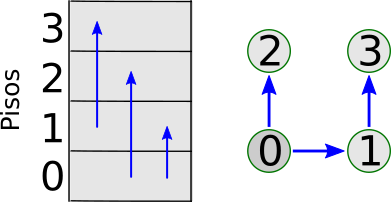
\includegraphics[width=4cm]{images/ej1/example.png}

    
    \caption{Problema ejemplo: n = 3, tres portales: (0,1) (0,2) (1,3)
    A la izquierda podemos ver el ''Pabellón'' representado, y a la derecha el grafo que lo representa.\label{grf:ex1-example}}
\end{figure}

Supongamos, entonces, que tenemos tan sólo 1 nodo. En este caso, el único camino posible es el camino vacío, y por lo tanto el mismo es el máximo. Por otro lado, si tenemos $n + 1$ nodos, y poseemos las longitudes $L_i$ de los caminos máximos que conectan al piso inicial con cada uno de los $n$ nodos anteriores, observemos que la longitud del camino máximo hasta el nodo $n + 1$ es exactamente:

$$L_{n + 1} = max\{L_k + 1 : k \in \mathbb{N}, k \leq n, \text{el nodo } k \text{ está conectado con } n + 1 \text{ y existe camino desde } 0 \text{ hasta } k\}$$

Es decir, la longitud del camino máximo que conecta al nodo inicial con el nodo $n + 1$ es la longitud del camino máximo que conecta al nodo inicial con algún nodo anterior al mismo que esté conectado con $n + 1$, sumándole 1 (por la arista adicional que tendríamos que utilizar). Observemos que esto es posible únicamente por la condición del orden que mencionamos anteriormente, ya que en general la condición de optimalidad no se cumple para camino máximo, como vimos en la teórica.

\begin{lemma}
El camino máximo en el sentido descripto cumple con el principio de optimalidad.
\end{lemma}

\begin{proof}
Sea $C$ un camino de longitud máxima que une al nodo inicial con el nodo $n$, y supongamos que hay algún fragmento del camino que no es máximo, llamémosle a este fragmento $H$. Entonces, existe algún fragmento $J$ que une a los mismos nodos que $H$ y cumple que $|J| > |H| \iff |J| - |H| > 0$. Tomemos entonces al camino $C'$ como el que resulta de reemplazar en $C$ al fragmento $H$ por el fragmento $J$, entonces:

$$|C'| = |C| - |H| + |J| > |C|$$

Por lo tanto $C'$ es un camino con longitud mayor a $C$. Absurdo, pues $C$ era un camino de longitud máxima. Observemos que, sin decirlo, estamos utilizando muy fuertemente que no hay ciclos en el digrafo, ya que si los hubiese estaríamos intentando demostrar el principio de optimalidad para camino más largo sin pesos, donde no tenemos la noción de independencia entre soluciones que sí tenemos de esta forma.
\end{proof}

En términos de la programación, elegimos utilizar la versión iterativa bottom up del algoritmo, donde básicamente la idea es recorrer un nodo y actualizar los vecinos, de forma similar al recorrido de un BFS: dado un nodo $i$, recorremos todos los posibles nodos a los que pueda tener un portal $j \in \{i + 1, .., n\}$, y si estamos conectados intentamos actualizar la distancia máxima hasta ese nodo. De cualquier forma, cabe destacar que sólo los nodos $i$ que sean alcanzables desde el comienzo deberían ser actualizados, ya que si no podríamos actualizar de forma errónea la distancia. Si bien no está reflejado en el pseudocódigo del algoritmo \ref{alg:ex1}, en la práctica decidimos utilizar un jagged array para representar la matriz de adyacencia, ya que la condición de que los nodos sólo conecten hacia arriba nos determina automáticamente la orientación de las aristas, en el caso de haberlas, y por lo tanto no necesitamos toda la información, basta con sólo aquello que está arriba de la diagonal. Veamos, entonces, que el algoritmo es correcto:

\begin{definition}
Decimos que un piso es alcanzable cuando existe un camino desde el piso inicial hasta él.
\end{definition}

\begin{lemma}
Los nodos no alcanzables no alteran el camino máximo desde 0 a n.
\end{lemma}

\begin{proof}
Supongamos que un nodo no alcanzable sí altera el camino máximo entre los nodos 0 y n. Entonces, el nodo no alcanzable debe pertenecer al mismo. Absurdo, pues si pertenece al camino máximo entonces es alcanzable a través del sub-camino que lo une con 0.
\end{proof}

\begin{lemma}
Al comenzar la $i$-ésima iteración del ciclo externo, si el nodo $i$ es alcanzable, $best[i]$ tiene la longitud del camino más largo de $0$ a $i$.
\end{lemma}

\begin{proof}
Sea n la cantidad de pisos e $i$ el número de piso, tal que $0 \leq i < n$. \\
Por inducción en $i$. \\

Cuando $i = 0$, al iniciar la primera iteración, $best[0] = 0$. Esto es lo esperable, dado que por definición: el camino que comienza en un nodo y termina en sí mismo tiene longitud 0. \\

Luego, siendo $i > 0$, supongamos que el lema vale para todo $0 \leq k < i$, estando $k$ conectado con $i$. Esto significa que para todo nodo $k$, al comenzar la $k$-ésima iteración, el algoritmo llevaba guardado en $best[k]$ la longitud del camino máximo de $0$ a $k$ y luego del segundo ciclo los valores de todos los vecinos de $k$ fueron actualizados tomando el máximo entre el valor ya guardado y $best[k]+1$ (por utilizar la arista de $k$ a su vecino). Como dijimos que $i$ es vecino de $k$ y para cada $k$ estamos guardando en $best[i]$ el valor máximo entre el ya guardado y $best[k]+1$, en particular, al terminar de iterar por los $k$ nodos, obtuvimos el máximo entre todos los $best[k]+1$ en $best[i]$. Finalmente, podemos asegurar que ésta es la longitud máxima de $0$ a $i$ porque debe ser el máximo de todos los caminos que comienzan en 0 y llegan a él; y, por la condición de orden que mencionamos anteriormente en la demostración, todos estos caminos pasan únicamente por nodos inferiores a él y hemos recorrido todos.
\end{proof}

Finalmente, dado que el último nodo es alcanzable por definición del problema, por los lemas \textbf{1.0.2, 1.0.3}, sabemos que al retornar $best[floors-1]$ estamos devolviendo la longitud de un camino máximo del primer nodo al último.

\subsection{Complejidad y experimentación}

Como el algoritmo descripto es el único utilizado en la resolución del problema, y como pueden apreciarse las complejidades de las operaciones en el pseudocódigo del algoritmo \ref{alg:ex1}, lo único que queda por analizar son los dos ciclos que contiene y determinar los mejores y peores casos. Cabe destacar, que no contabilizamos aún el algoritmo que se ocupa de construir la matriz, sin embargo, el mismo toma $Theta(n^2)$ pues lo único que hace es pedir la memoria y rellenar las entradas con los valores correspondientes; y por lo tanto la complejidad asintótica del algoritmo es en todos los casos $\Omega(n^2)$. Veamos qué sucede con el algoritmo de resolución en sí.

Se puede ver que el algoritmo contiene un ciclo principal, que siempre realiza $n$ iteraciones; dentro de él se tiene un condicional y un ciclo interno, y éste último se ejecutará en caso de no cumplirse la guarda del condicional previo. Dado que el ciclo principal se ejecuta siempre $n$ veces, centraremos el análisis en el ciclo secundario, veremos en qué casos se realiza y cómo afecta la complejidad en cada caso.

En peor caso, el ciclo secundario toma $n$ iteraciones y se realiza para cada iteración del ciclo principal. Esto sucede cuando cada piso está conectado a todos los pisos más altos que él, porque para cada iteración del ciclo principal la guarda del condicional no se cumple (dado que el primer piso siempre va a poder alcanzar al piso actual), con lo cuál se ejecuta el ciclo secundario. Éste itera desde el próximo piso al actual hasta el último piso, lo cuál nos permite acotar por $n$ cantidad de iteraciones y dejando así la complejidad en peor caso como $O(n^2)$.

\begin{figure}
    \centering
    
    \begin{tabular}{cccc}
        \subfloat{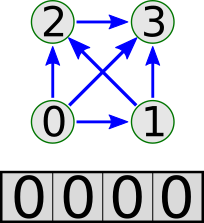
\includegraphics[width=3cm]{images/ej1/worstcase/00.png}} &
        \subfloat{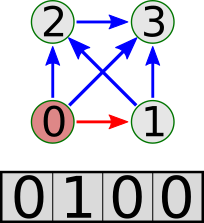
\includegraphics[width=3cm]{images/ej1/worstcase/01.png}} &
        \subfloat{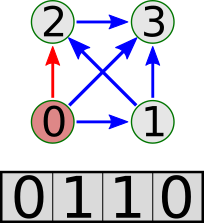
\includegraphics[width=3cm]{images/ej1/worstcase/02.png}} &
        \subfloat{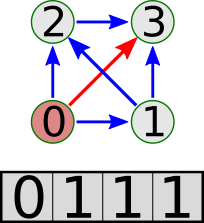
\includegraphics[width=3cm]{images/ej1/worstcase/03.png}} \\
        
        \subfloat{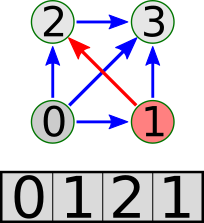
\includegraphics[width=3cm]{images/ej1/worstcase/12.png}} &
        \subfloat{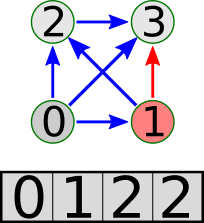
\includegraphics[width=3cm]{images/ej1/worstcase/13.png}} &
        \subfloat{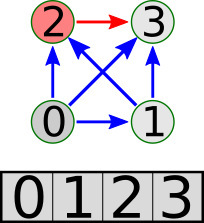
\includegraphics[width=3cm]{images/ej1/worstcase/23.png}} &
        \subfloat{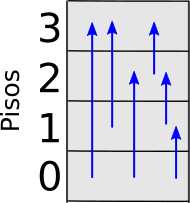
\includegraphics[width=3cm]{images/ej1/worstcase/floors.png}}
    \end{tabular}
    
    \caption{Ejemplo de una corrida de peor caso para el ejercicio 1. El arreglo de abajo representa a best en el pseudocódigo. No incluimos reachable por no parecernos necesario a la comprensión. 
    La ultima imagen muestra el ''pabellón'' representado\label{grf:ex1-worst}}
\end{figure}

Por otro lado, el mejor caso debería minimizar la cantidad de ejecuciones del ciclo secundario. Notemos que esto sucede cuando el único portal existente es el que va del primer piso al último piso, ya que esto implicaría que todos los pisos intermedios no serían alcanzables, forzando la guarda del if a saltear la iteración. Cuando esto sucede, las únicas iteraciones que realizaremos serán la primera (porque el nodo inicial es alcanzable trivialmente) y la última (porque el nodo final es alcanzable a través del único portal que conecta al inicial con el mismo). En la primera iteración, la guarda del if no se cumple y el ciclo en cuestión itera desde el piso 1 hasta el último, tomando $O(n)$ pasos. Por último, en la última iteración no se cumple la guarda del condicional pero dado que se trata del último piso tampoco se cumple la guarda del ciclo y por eso éste no corre. Habiendo dicho esto, podemos ver que el ciclo principal toma $n$ iteraciones, y cada una tiene complejidad $O(1)$ excepto la primera que es $O(n)$, por ende este caso toma $O(n)$. Sin embargo, el algoritmo para construir la matriz tomaba $\Theta(n^2)$, por lo que tenemos que el nuevo algoritmo tomará $O(n^2 + n) = O(n^2)$.

\begin{figure}
    \centering
    
    \begin{tabular}{cccc}
        \subfloat{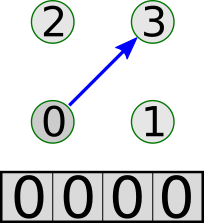
\includegraphics[width=3cm]{images/ej1/bestcase/00.png}} &
        \subfloat{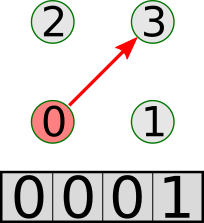
\includegraphics[width=3cm]{images/ej1/bestcase/01.png}} &
        \subfloat{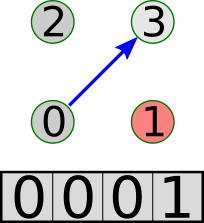
\includegraphics[width=3cm]{images/ej1/bestcase/10.png}} &
        \subfloat{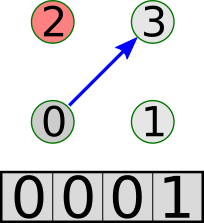
\includegraphics[width=3cm]{images/ej1/bestcase/20.png}}
    \end{tabular}
    
    \caption{Ejemplo de una corrida de mejor caso para el ejercicio 1. El arreglo de abajo representa a best en el pseudocódigo. No incluimos reachable por no parecernos necesario a la comprensión. \label{grf:ex1-best}}
\end{figure}

\pagebreak

En términos de la experimentación, la generación de mejor caso no nos deja opción en términos de qué es lo que queremos generar: por el enunciado, todo piso tiene exactamente una arista dirigida hacia algún piso superior, y sabemos que en el mejor caso el primer piso tiene exactamente una conexión con el último piso. Fuera de eso, los otros pisos deberán estar conectados entre sí, pero observemos que el costo de crear estas conexiones está contemplado en el $\Theta(n^2)$ que utilizamos para la entrada y salida, y por ende no nos lleva a un cambio sustancial de complejidad como para que tenga sentido experimentar qué pasa. Por otro lado, el peor caso tampoco nos deja opción: cada piso debe tener una arista dirigida apuntando hacia todos los pisos superiores al mismo, por lo que la instancia queda unívocamente determinada por la cantidad de pisos (y por ende lo único con lo que podemos experimentar es la cantidad de pisos).

Con respecto a los casos aleatorios, primero aseguramos que haya solución generando una arista que conecte el piso 0 con el N. Luego por cada piso i, decidimos generar una cantidad aleatoria X de portales entre i y N. Luego de determinar X, se decide si un portal o no se va a crear con probabilidad $0.25$. Si se decide crear el portal, se elige un número $z$ entre $i+1$ y $N$ y se crea el portal $(i, z)$. No importa que haya repetidos, ya que usamos un conjunto para guardar los portales en el código de generación, y el conjunto por definición no permite repeticiones.

Con respecto a los resultados, la figura \ref{grf:ex1} nos muestra que efectivamente la complejidad es como suponíamos: en ambos casos, dividiendo el tiempo de ejecución por su complejidad acorde al tamaño del problema en esa instancia, se termina convergiendo hacia constantes como era de esperarse, y de hecho el mejor caso tiende a una constante más pequeña que el peor caso, indicando que efectivamente hemos distinguido bien los distintos casos. Más aun, el gráfico que incluye al caso aleatorio muestra que la complejidad del mismo está claramente entre medio de las cotas superior e inferior, como es de esperarse; cabe destacar, sin embargo, que los tiempos del caso aleatorio tienden hacia los de el mejor caso, por lo que asumimos que hay un bias en el generador de casos hacia grafos con poca densidad de aristas.

Las grandes variaciones para las instancias pequeñas se deben a que factores físicos como estado de caché del procesador y carga del sistema operativo pasan a ser mucho más influyentes que la complejidad de la solución en sí. En el caso aleatorio, las variaciones que observamos suponemos que debe estar relacionado con las instancias en las que haya habido un camino muy corto de portales que conecten al nodo inicial con el final.

\begin{figure}
\centering
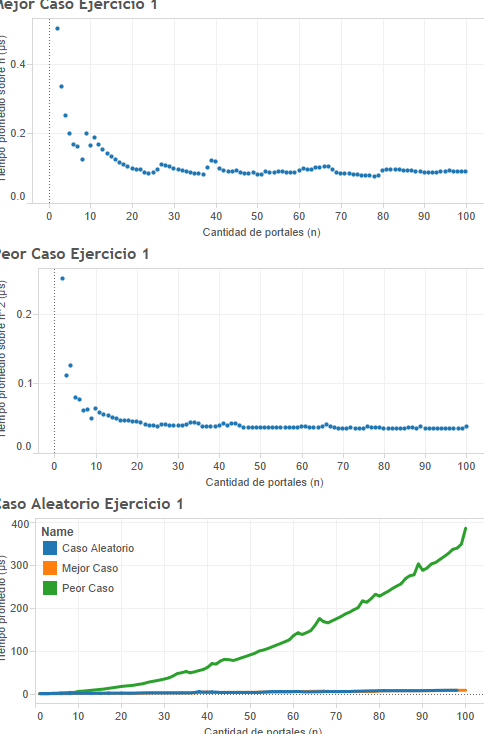
\includegraphics[width=10cm]{ex1}
\caption{El estadístico que tomamos es la media alfa podada de 100 corridas con $\alpha = 0.10$, que nos permite evitar algunos outliers. En ambos casos estamos graficando a las funciones sobre las complejidades esperadas. \label{grf:ex1}}
\end{figure}

\vspace{2cm}
\pagebreak
\newpage

\section{Problema 2}
\subsection{Resolución y correctitud}

\begin{algorithm}[h!]
\caption{Algoritmo de Breadth First Search. $n$ es la cantidad de vértices del grafo, $m$ la cantidad de aristas. \label{alg:bfs}}

\begin{algorithmic}[h!]
\Procedure{BFS}{$G$ grafo, $t$ nodo final}
\State queue $\gets$ Cola vacia \Comment $O(1)$
\State distances $\gets$ Arreglo de tamaño $|G.V|$ inicializado a -1 \Comment $O(n)$

\State distances[0] = 0 \Comment $O(1)$
\State queue.push(0) \Comment $O(1)$

\While{queue no esté vacia} \Comment $O(n + m)$
    \State current $\gets$ queue.pop() \Comment $O(1)$
    
    \For{neighbor vecino de current} \Comment $O(dg(current))$
        \If{distance[neighbor] $=$ -1} \Comment $O(1)$
            \State distance[neighbor] $\gets$ distance[current] + 1 \Comment $O(1)$
            \State queue.push(neighbor) \Comment $O(1)$
        \EndIf
        
        \If{neighbor $=$ t} \Comment $O(1)$
            \State return distances[neighbor] \Comment $O(1)$
        \EndIf
    \EndFor
\EndWhile
\EndProcedure
\end{algorithmic}
\end{algorithm}

\vspace{10em}
A priori, leer el enunciado deja claro que la solución debe involucrar tomar el camino mínimo que conecte a la posición inicial con la posición final (el aula). El primer modelo al que llegamos involucraba tener un nodo por cada posición que tuviese un portal, la posición inicial, y la posición final, y conectar cada uno de estos nodos con los otros que estén en el mismo piso (tomando como peso la cantidad de segundos que tardaríamos en recorrer el trayecto) y con los nodos a los que un portal pueda llevarlo (poniéndole peso 2 a cada arista, que simboliza una vez más la cantidad de tiempo). Con este modelo, queda claro que el problema del enunciado se traduce en calcular el camino mínimo que une a la posición inicial con el aula de algoritmos. Sin embargo, un análisis rápido de complejidad temporal muestra que este modelado no admite una solución que esté cumpla el enunciado utilizando los algoritmos que vimos en la clase, y por lo tanto rápidamente lo descartamos.

Encontramos, entonces, otro modelo posible, basado en transformar el modelo recién expuesto: crear un nodo por cada posición posible (de esta forma tendríamos $NL$ nodos) y conectar todos los que estén en el mismo piso con peso 1 en las aristas, simbolizando que tardamos 1 segundo en movernos de una posición a otra; además, si hay un portal que conecta una posición con otra, agregamos un ''nodo fantasma'' en el medio, y conectamos el nodo a los dos extremos del portal con peso 1. Esta idea del ''nodo fantasma'' es para lograr eliminar la noción de peso que tenían los ejes en el grafo original, obteniendo finalmente un grafo con peso 1 global para todas las aristas.\par

De esta forma, tenemos exactamente $NL + P$ nodos (uno por posición y un ''nodo fantasma'' por portal) y un total de $N (L-1) + 2P$ aristas. Observemos que en este nuevo grafo, el hecho de tener pesos uniformes nos permite calcular el camino mínimo utilizando BFS como vimos en la teórica; dado que la complejidad temporal de BFS es $O(m + n)$, tenemos que en particular para este grafo se convierte en $O(NL + P + N (L-1) + 2P) = O(NL + P)$, y por lo tanto estaríamos cumpliendo con la complejidad pedida por el enunciado.

\begin{figure}
    \centering
    
    \begin{tabular}{ccc}
        \subfloat{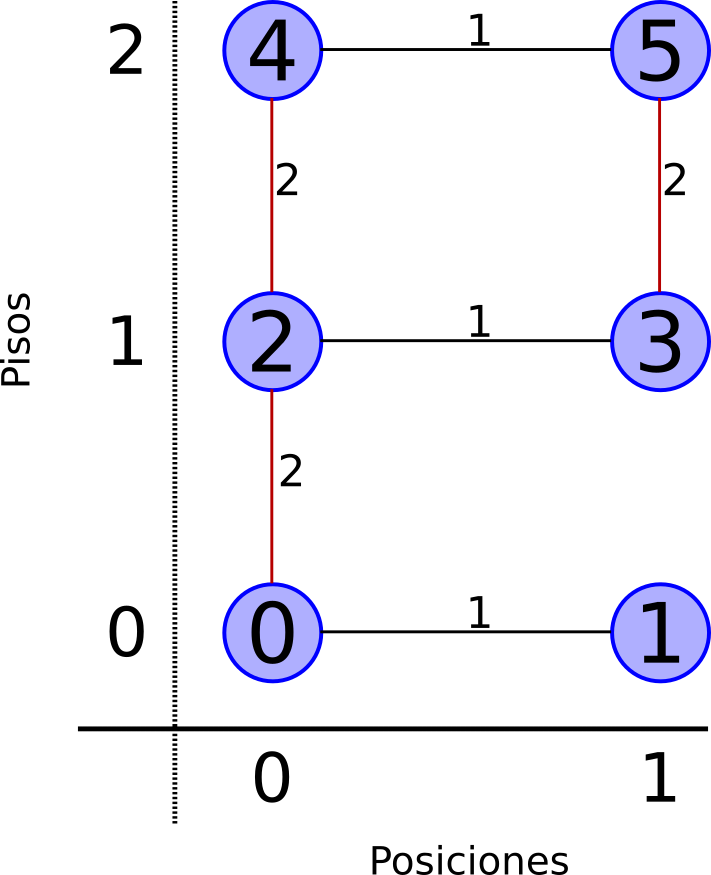
\includegraphics[width=4cm]{images/ej2/example_normal.png}} &
        \subfloat{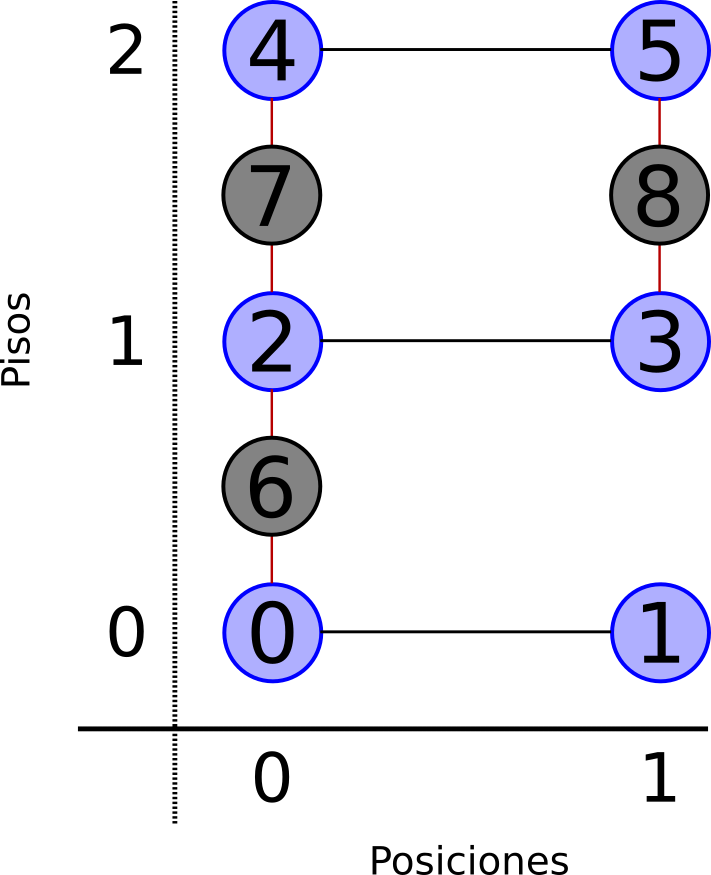
\includegraphics[width=4cm]{images/ej2/example_expanded.png}}
    \end{tabular}
    
    \caption{A la izquierda podemos ver el grafo que modela el problema mas intuitivamente ($G$) y a la derecha el grafo ($G'$) transformado al modelo propuesto sin pesos (los ''nodos fantasma'' se pueden ver en color gris)
    Las aristas rojas representan a los portales, las negras al costo de caminar entre cada posición dentro de un piso\label{grf:ex2-example}}
\end{figure}
    

Observemos, además, que asumiendo que tenemos la cantidad de nodos que precisamos crear, tomar una representación utilizando listas de adyacencia nos permite que generar el grafo a partir de los datos tenga un costo de $O(NL)$ para crear todos los nodos correspondientes a las posiciones y sus conexiones, y $O(P)$ para agregar los nodos fantasma de los portales, junto con sus aristas. Es decir, tendríamos que en conjunto todo el algoritmo correría en $O(NL + P)$.

Dicho más formalmente, la transformación que realizamos es dada una arista $e = (u, v)$ con peso $p(e)$, la reemplazamos por nodos $n_1, ..., n_{p(e)-1}$ con aristas $(n_i, n_{i+1})$ donde $i \in {1, ..., p(e) - 2}$ y dos aristas $(u, n_1), (n_{p(e)-1}, v)$ que nos permiten conectar los nuevos nodos a las posiciones. Además, agregamos nodos por cada posición y los conectamos con sus posiciones vecinas. De aquí en adelante, llamaremos $G = (V, E)$ al grafo inicial, y $G' = (V', E')$ al grafo transformado. Supongamos entonces que un camino en $G$ pasa por una arista $e \in E$ con peso $p(e)$, entonces transformar a las aristas como dijimos anteriormente nos dará un camino en $G'$. Es decir, para cada camino en $G$ podemos obtener un camino en $G'$; aunque la vuelta no necesariamente vale, dado que un camino que pase por entre medio de los nodos agregados no tiene su correspondiente en $G$ (cabe destacar, cualquier camino que no tenga esta condición sí va a poder volver la transformación hacia atrás).

\begin{definition}
Decimos que un $C'$ camino en $G'$ es recuperable si hay algún camino en $G$ que podamos transformar en él (es decir, si podemos volver la transformación hacia atrás). Observemos que si tenemos un camino $C$ en $G$, y lo transformamos en un camino $C'$ en $G'$ con el procedimiento expuesto, el camino $C'$ es recuperable, y su camino correspondiente es $C$; es decir, la transformación de caminos es "inversible".
\end{definition}

\begin{definition}
Dado $C$ un camino en $G$, llamamos $P(C)$ al peso total de recorrer el camino, y $|C|$ a la longitud del mismo.
\end{definition}

\begin{lemma}
$C$ es un camino de peso mínimo en $G$ sí y sólo sí $C'$ es un camino de longitud mínima recuperable en $G'$
\end{lemma}

\begin{proof}

$\implies$ ) Sea $H$ otro camino en $G$, $H'$ su correspondiente en $G'$. Tenemos que $P(C) = |C'|$ y $P(H) = |H'|$ por la transformación que realizamos, y además $P(C) \leq P(H)$ por ser camino mínimo. Es decir, $|C'| \leq |H'|$; además, ambos caminos son recuperables (y $H'$ recorre todos los caminos recuperables).

$\impliedby$ ) Supongamos que existe algún otro camino $H$ en $G$, con pesos menores a $C$. Tenemos que $p(H) = |H'|$, y además $p(C) = |C'| > P(H) = |H'|$. Es decir, $|C'| \geq |H'|$, contradiciendo la hipótesis que $C'$ es un camino de longitud mínima recuperable en $G'$.
\end{proof}

\begin{lemma}
Si $u, v$ son nodos en $G$, y encontramos un camino $C'$ que los une en $G'$, $C'$ es recuperable
\end{lemma}

\begin{proof}
Por inducción en la longitud de $C'$. Si $|C'| = 0$, $u = v$ y el camino vacío es recuperable.
Supongamos que vale para todo camino de longitud menor o igual a $r$, veamos que vale cuando $|C'| = r + 1$. Desde $u$, tenemos una arista $e$ que lo conecta con algún otro nodo $z$. Tenemos, entonces, varias posibilidades:

\begin{enumerate}
\item $z$ es un nodo que corresponde a un portal, en cuyo caso $z$ está conectado con algún otro nodo $w$ que está originalmente en $G$. Entonces, si tomamos el subcamino de $C'$ que comienza en $w$ y termina en $v$, por hipótesis inductiva es recuperable. Agregando, entonces, a las aristas que unen $u$ con $w$, tenemos un camino recuperable que une $u$ con $v$.

\item $z$ es un nodo que corresponde a una posición que ya estaba en el grafo anterior, entonces el subcamino de $C'$ que une $z$ a $v$ es recuperable por hipótesis inductiva, y tan solo tenemos que agregar a la arista $e$, que también debe pertenecer al grafo $G$. 

\item $z$ es un nodo que corresponde a una posición que no estaba en el grafo anterior, en cuyo caso tenemos una cadena de posiciones que nos debe llevar a la próxima posición que tenga un portal (por construcción del grafo), además, todas estas posiciones se corresponden con una única arista en el grafo original. Si tomamos entonces al próximo nodo en $G'$ que tenga un portal, el subcamino de $C'$ desde el mismo hasta $v$ es recuperable por hipótesis inductiva, y todos los nodos intermedios que unen a $v$ con el nodo del portal son reconstruibles por el proceso explicado, entonces el camino total es reconstruible.
\end{enumerate}
\end{proof}

Cabe destacar, entonces, que estos lemas nos permiten afirmar que si encontramos un camino de longitud mínima en $G'$, recuperarlo a un camino de peso mínimo en $G$ es posible y, más todavía, la longitud del mismo es equivalente al peso del camino mínimo en $G'$. Entonces, podemos aplicar BFS para obtener el camino de longitud mínima en $G'$ y con eso conseguir el peso del camino mínimo en $G$, que era nuestro objetivo original.

\subsection{Complejidad y experimentación}

Veamos que tras modelar nuestro grafo se obtiene que, independientemente de los portales dados, nuestro pre-procesamiento genera un nodo por cada metro de cada piso del edificio, por lo que tenemos $NL$ nodos y hasta este momento una complejidad de $O(NL)$. Luego veremos que por cada conexión entre portales, agregamos un nodo intermedio entre los dos extremos de la conexión, por lo que ahora tendremos $NL+P$ nodos, con $P$ la cantidad de portales, formando así una complejidad de pre-procesamiento de $O(NL+P)$. Notemos que nuestro algoritmo termina apenas se evalúa un nodo que tenga como vecino al último metro del último piso -de ahora en más, nodo 'fin'-, habiendo dicho esto, centraremos nuestro análisis en los portales dados porque es lo único que logrará variar la cantidad de iteraciones que tomará para llegar a dicho nodo. \\

Ahora bien, si quisiéramos obtener el mejor caso, sería minimizando la cantidad de portales porque habría menos nodos a considerar a la hora de encolar, chequear sus vecinos e iterar a través de ellos, además de un preprocesado menos costoso. Dado que es condición necesaria del problema que exista un camino posible, necesitamos que exista al menos un camino del piso 0 al piso n, y para minimizar dicho camino de portales podemos considerar un portal único que vaya desde el metro 0 del piso 0 al nodo 'fin' (metro $L$ del nodo $N$). En este caso (Figura \ref{grf:ex2-best}), en la primera iteración nuestro algoritmo encolará a los dos vecinos del metro 0 (el metro 1 y el portal intermediario que llevará al nodo 'fin'), luego al desencolar el portal intermediario iteraremos por su único vecino y dado que es el nodo 'fin' terminaremos la ejecución del algoritmo. Notemos que la resolución del camino mínimo propiamente dicha tomó tiempo constante en este caso, dado que no depende del largo de los pasillos $L$, ni de la cantidad de pisos $N$; sin embargo como contamos con el preprocesamiento antes mencionado, la complejidad se vuelve $O(NL+1)$, que es $O(NL)$.\\

\pagebreak
    
\begin{figure}
    \centering
    
    \begin{tabular}{ccc}
        \subfloat{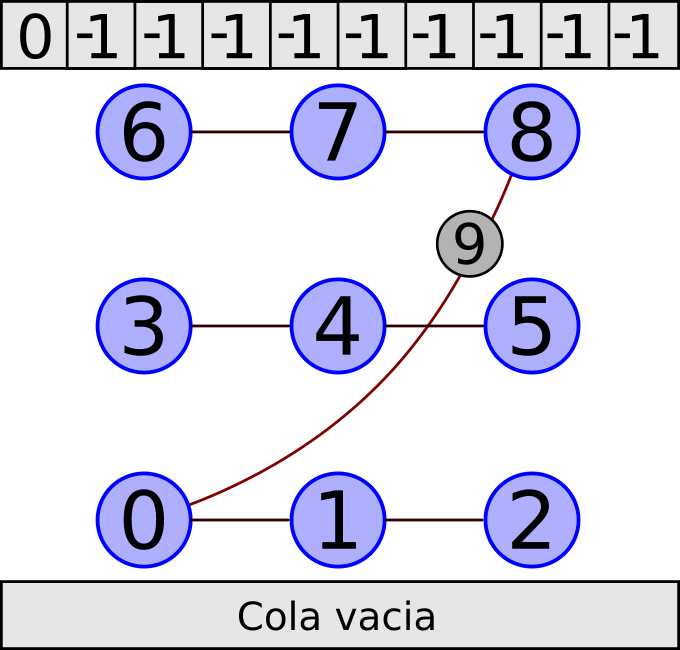
\includegraphics[width=4cm]{images/ej2/bestcase/00.png}} &
        \subfloat{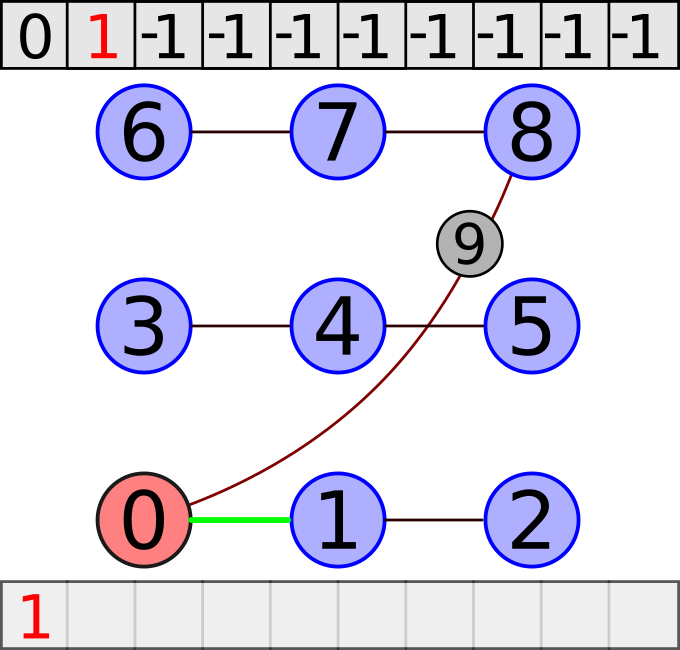
\includegraphics[width=4cm]{images/ej2/bestcase/01.png}} &
        \subfloat{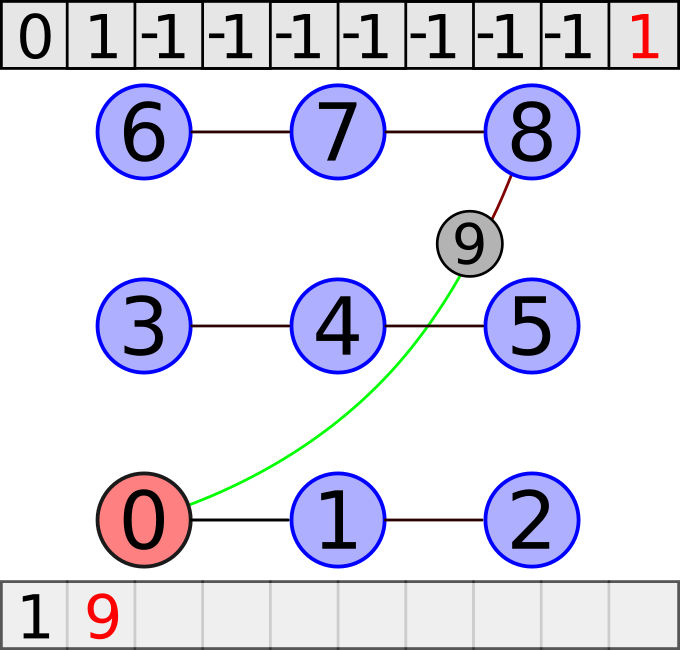
\includegraphics[width=4cm]{images/ej2/bestcase/09.png}} \\
        \subfloat{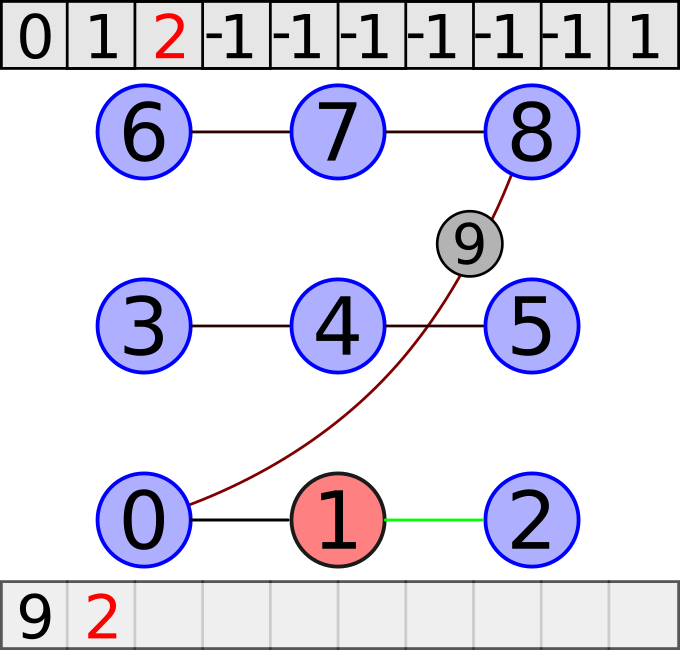
\includegraphics[width=4cm]{images/ej2/bestcase/12.png}} &
        \subfloat{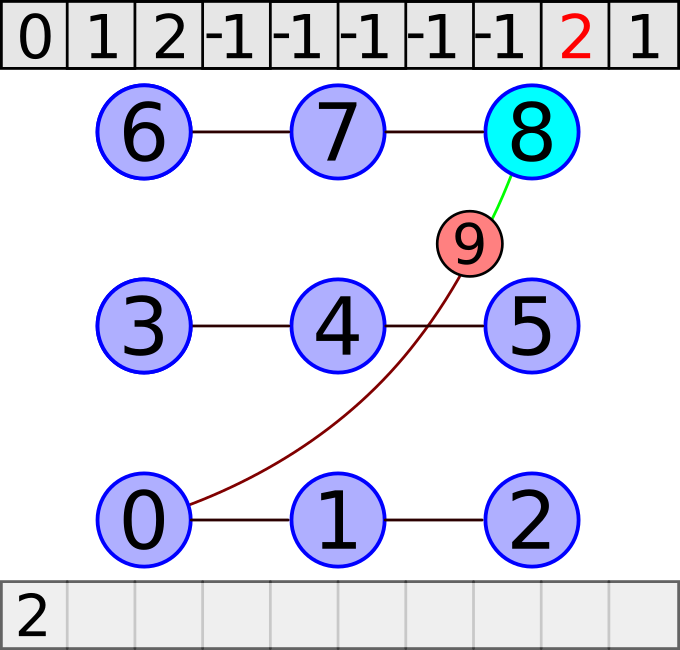
\includegraphics[width=4cm]{images/ej2/bestcase/98.png}}
    \end{tabular}
    
    \caption{Ejemplo de una corrida de mejor caso para el ejercicio 2. El arreglo de arriba representa el arreglo de distances del algoritmo, y el de abajo la cola utilizada. \label{grf:ex2-best}}
\end{figure}

Por otro lado, veamos que en peor caso (figuras \ref{grf:ex2-worst-1} y \ref{grf:ex2-worst-2}), la mayor cantidad de iteraciones se da cuando tengamos que pasar por todos los nodos para encontrar el camino mínimo que llega al nodo 'fin' y además cada nodo tenga la mayor cantidad de vecinos (para así maximizar la cantidad de iteraciones del ciclo interno); la única excepción a esto es el ante-último piso, ya que aquí todos los nodos tendrán que estar conectados con el metro 0 del último piso -dado que de lo contrario, estarían más cerca de llegar al nodo 'fin'.\\

Notemos que al momento de buscar maximizar la cantidad de vecinos de un nodo $n$ en el piso $i$, es necesario que $n$ esté conectado con todos los nodos del piso $i+1$ pero con ninguno superior a dicho piso, porque si lo estuviera, el algoritmo estaría aproximándose más rápidamente al portal que comunica con el último piso, y terminaría antes. De esta forma se tiene que el último piso tendrá un solo portal (en el metro 0), el anteúltimo piso tendrá $L$ portales (que comunican con el metro 0 del último piso), y todos los anteriores tendrán $L^2$ portales (cada metro del $i$-ésimo piso con todos los metros del $i+1$-ésimo piso). Con lo cuál la cantidad de portales será: $P = 1+L+(N-2)L^2$. \\

\pagebreak

\begin{figure}
    \centering
    
    \begin{tabular}{ccc}
        \subfloat{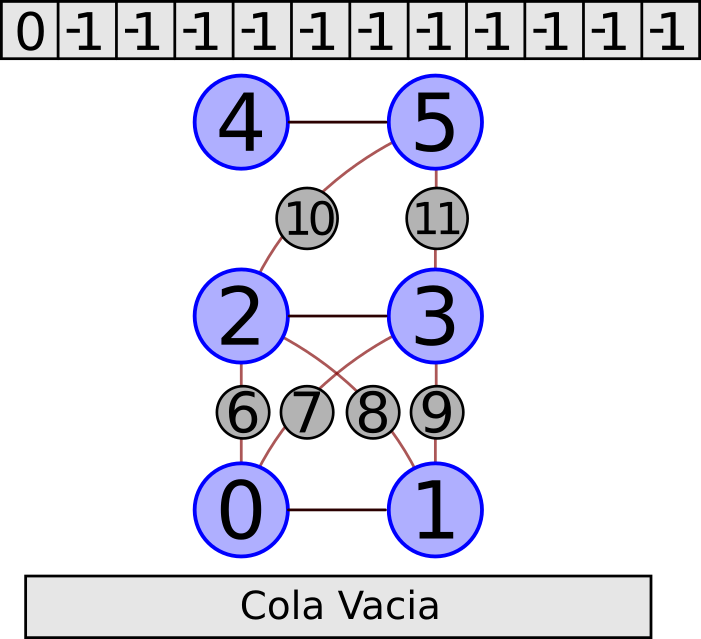
\includegraphics[width=4cm]{images/ej2/worstcase/00-00.png}} &
        \subfloat{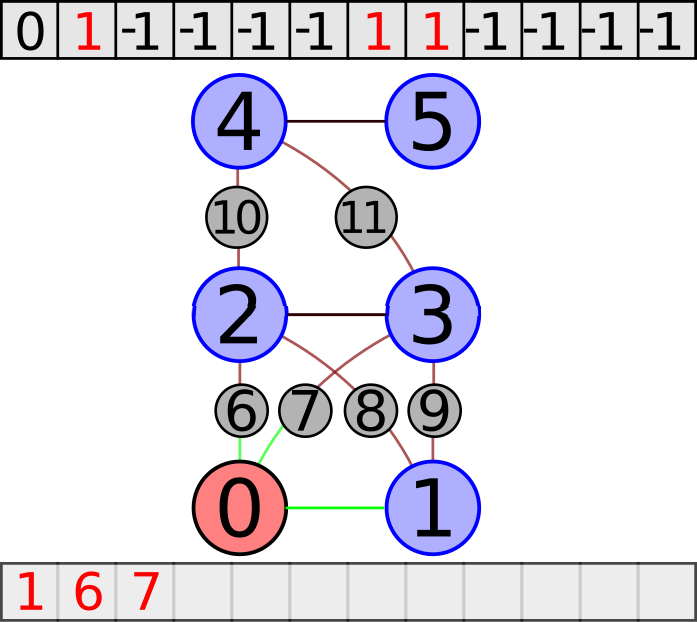
\includegraphics[width=4cm]{images/ej2/worstcase/01-0167.png}} &
        \subfloat{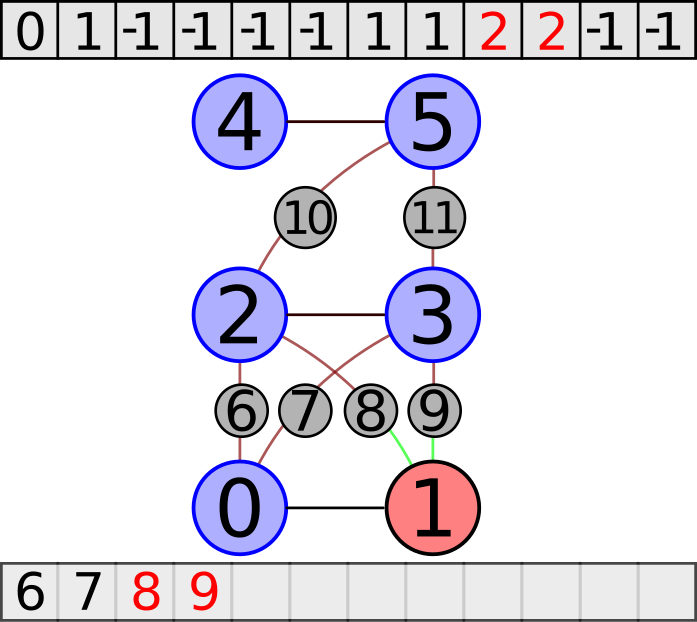
\includegraphics[width=4cm]{images/ej2/worstcase/02-189.png}} \\
        
        \subfloat{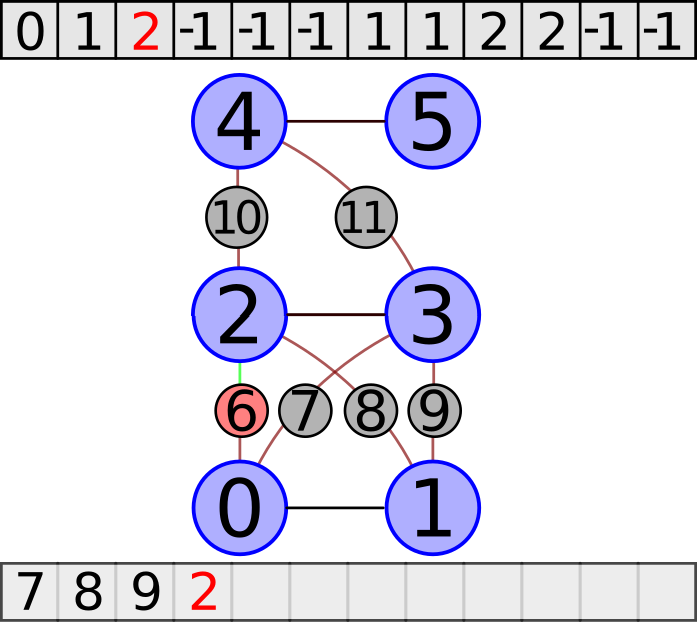
\includegraphics[width=4cm]{images/ej2/worstcase/03-62.png}} &
        \subfloat{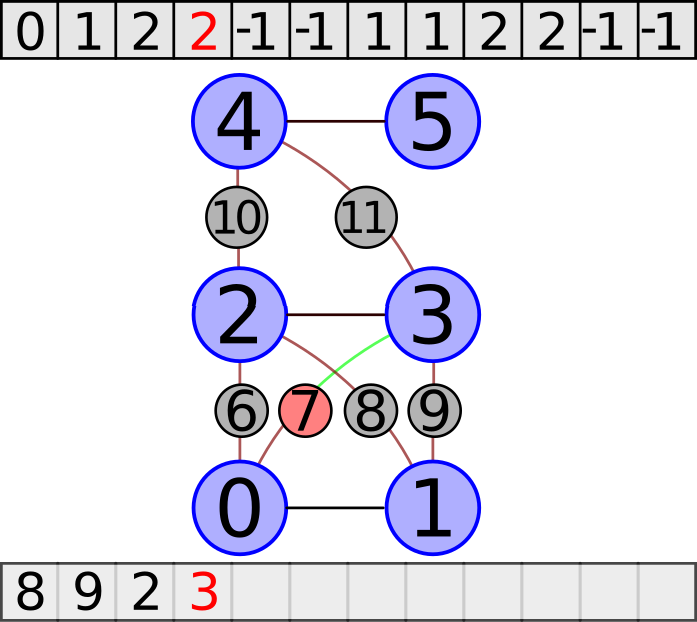
\includegraphics[width=4cm]{images/ej2/worstcase/04-73.png}} &
        \subfloat{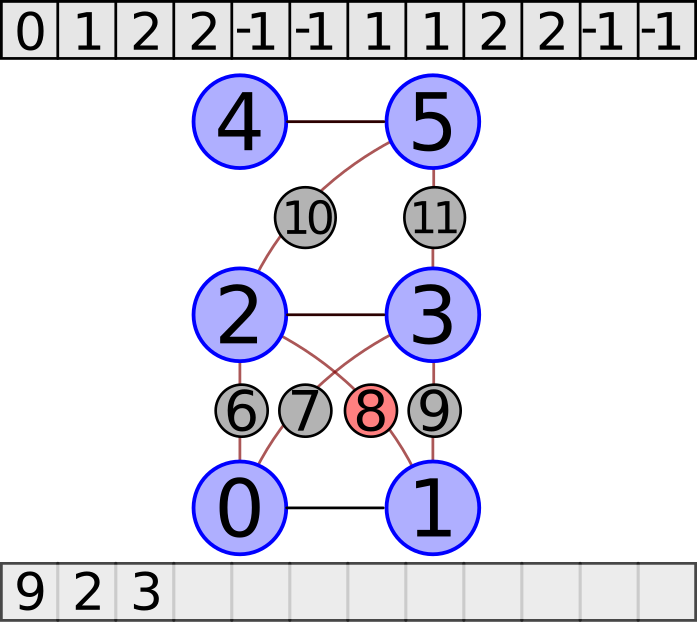
\includegraphics[width=4cm]{images/ej2/worstcase/05-8.png}} \\
        \end{tabular}
    
    \caption{Ejemplo de una corrida de peor caso para el ejercicio 2. El arreglo de arriba representa el arreglo de distances del algoritmo, y el de abajo la cola utilizada.(Parte 1)\label{grf:ex2-worst-1}}
\end{figure}

\begin{figure}
    
    \centering
    
    \begin{tabular}{ccc}
        \subfloat{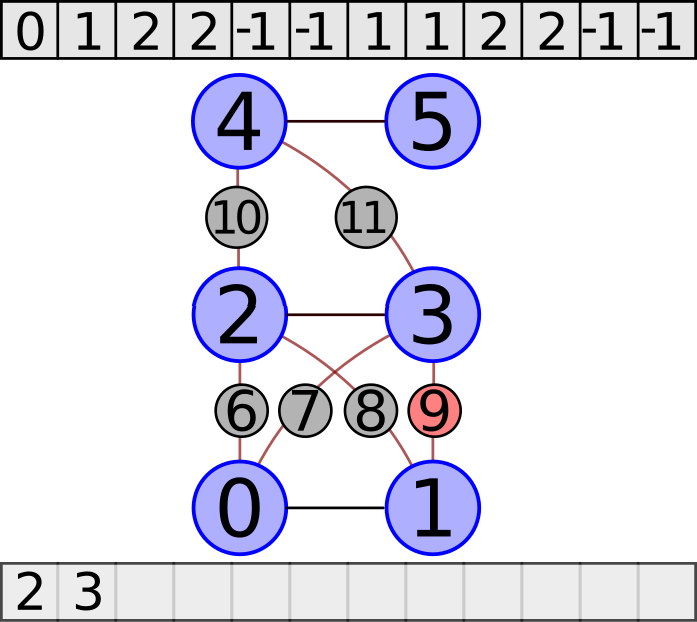
\includegraphics[width=4cm]{images/ej2/worstcase/06-9.png}} &
        \subfloat{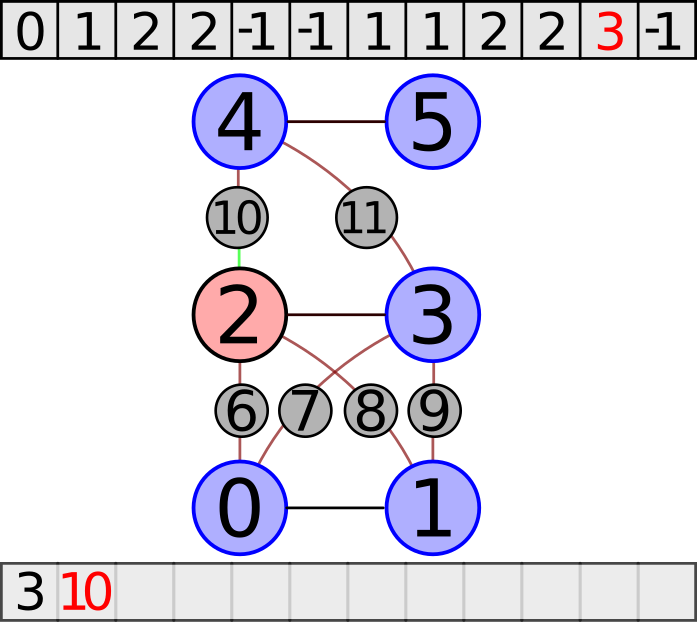
\includegraphics[width=4cm]{images/ej2/worstcase/07-210.png}} &
        \subfloat{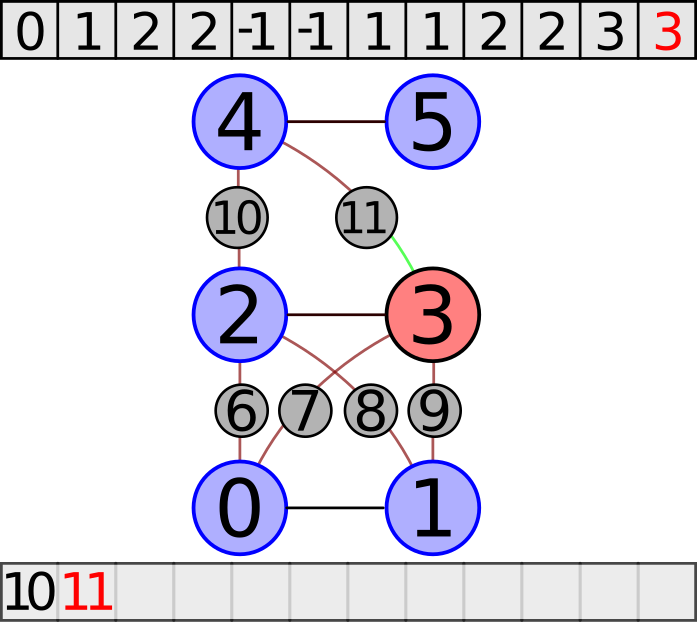
\includegraphics[width=4cm]{images/ej2/worstcase/08-311.png}} \\
        
        \subfloat{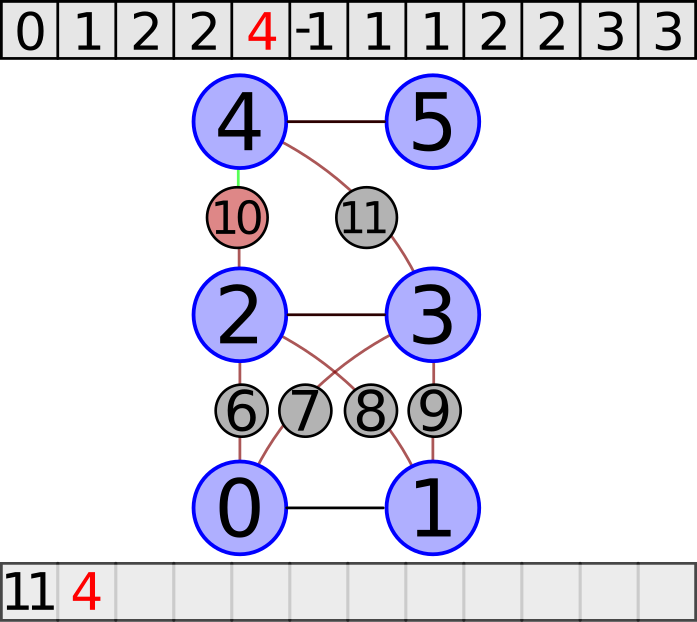
\includegraphics[width=4cm]{images/ej2/worstcase/09-104.png}} &
        \subfloat{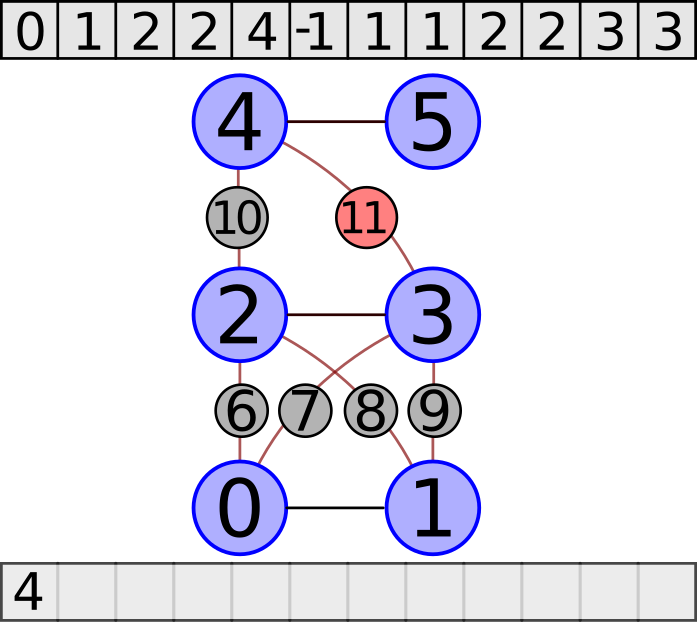
\includegraphics[width=4cm]{images/ej2/worstcase/10-11.png}} &
        \subfloat{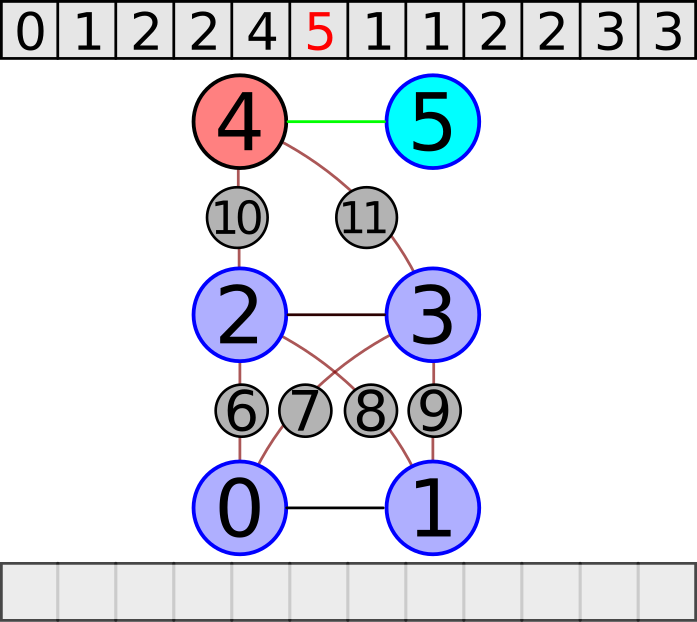
\includegraphics[width=4cm]{images/ej2/worstcase/11-45.png}}
    \end{tabular}
    
    \caption{Ejemplo de una corrida de peor caso para el ejercicio 2. El arreglo de arriba representa el arreglo de distances del algoritmo, y el de abajo la cola utilizada.(Parte 2)\label{grf:ex2-worst-2}}
\end{figure}

Para la generación de los casos de prueba, decidimos tomar $L = N$ para simplificar la comprensión de los gráficos (de cualquier forma, mirar los gráficos por separado da lo esperado, pero es más complicado de expresar los resultados).

Además, para probar de forma justa el mejor caso junto al peor caso decidimos que los casos de prueba tengan la misma cantidad de portales, es decir, el peor caso va a ser como fue descripto anteriormente (cada nodo se conecta con todos los del piso inferior y superior a través de portales, excepto el nodo 'fin'), y el grafo para el mejor caso va a ser igual pero simplemente conectando a través de un portal la posición 0 del piso 0 con el nodo 'fin'. De esta forma fijamos todas las las variables contempladas en la complejidad del algoritmo, y logramos comparar el desempeño del algoritmo equitativamente.

Para el caso aleatorio, lo que se decidió hacer es generar un árbol que conecte cada piso con el siguiente hasta N para asegurar que exista solución. Luego se generan pares de pisos y posiciones aleatorios, sin repetir ni violar el enunciado, hasta alcanzar la cantidad de portales generados en el mejor y peor caso, esto lo hacemos para poder comparar equitativamente los tres casos, fijando N, L y P, lograremos comparar el desempeño del algoritmo exclusivamente.
Observemos que el tiempo de corrida de los casos aleatorios es muy cercana al mejor caso, indicándonos que nuestra elección de mejor y peor caso fue acertada, y es lógico pensar que el caso aleatorio se acerca mucho mas al mejor caso que al peor, ya que eligiendo aleatoriamente conexiones es altamente improbable generar un grafo que cumpla las condiciones del peor caso (que los nodos de un piso conecten como máximo con el siguiente piso) y de hecho, con que solo un nodo logre ir a un piso mucho mas alto a través de un portal, recortara la cantidad de iteraciones de forma significativa.

En la figura \ref{grf:ex2} que tanto el mejor caso como el peor caso tienden a constantes, implicando que el crecimiento asintótico efectivamente es como esperábamos.

\begin{figure}
\centering
\centerline{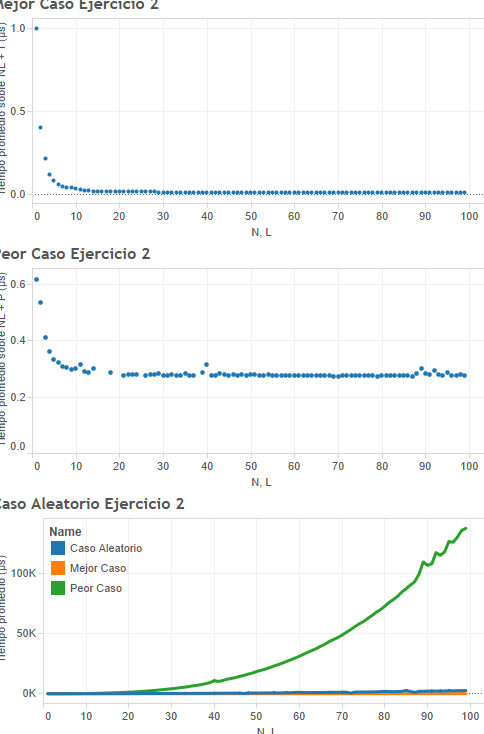
\includegraphics[width=10cm]{ex2}}
\caption{El estadístico que tomamos es la media alfa podada de 100 corridas con $\alpha = 0.10$, que nos permite evitar algunos outliers. En ambos casos estamos graficando a las funciones sobre las complejidades esperadas. Como el crecimiento del peor caso es cúbico, el caso aleatorio y el mejor caso se ven casi iguales comparados con el peor caso.\label{grf:ex2}}
\end{figure}


\pagebreak

\section{Problema 3}

\subsection{Resolución y correctitud}

La resolución del tercer ejercicio depende básicamente de darse cuenta de las pistas que nos da el enunciado: dado el modelo del problema que nos determina el enunciado, el requerimiento de que no haya ciclos en el grafo de salida se traduce literalmente en que el mismo sea un árbol. Más todavía, el requerimiento de que la diferencia de la suma sea mínima se traduce literalmente en la idea intuitiva de buscar el árbol que más distancia cubra en total, minimizando la cantidad de metros de pasillos a cerrar (y por lo tanto minimizando el costo de cerrarlos).

Como vimos en clase, el concepto análogo pero minimizando la distancia es el del árbol generador mínimo, y ya conocemos los algoritmos de Kruskal y de Prim para encontrarlo; por lo tanto, supusimos que probablemente sea posible modificar los algoritmos que ya conocíamos para resolver el nuevo problema de árbol generador máximo de forma eficiente:

\begin{lemma}
Sea $G = (V, E)$ un grafo conexo con pesos en los ejes determinados por $p : E \to \mathbb{R}$. Un árbol generador mínimo con función de pesos $q : E \to \mathbb{R} / q(e) = -p(e)$ es un árbol generador máximo con función de pesos $p$.
\label{pr:agm}
\end{lemma}

\begin{proof}
Sean $T = (V, E_T)$ un árbol generador mínimo con respecto a $q$ y $R = (V, E_R)$ un árbol generador. Tenemos, entonces, que

\begin{align*}
\sum_{e \in E_T} q(e) &\leq \sum_{e \in E_R} q(e)\\
\sum_{e \in E_T} -p(e) &\leq \sum_{e \in E_R} -p(e)\\
-\sum_{e \in E_T} p(e) &\leq -\sum_{e \in E_R} p(e)\\
\sum_{e \in E_T} p(e) &\geq \sum_{e \in E_R} p(e)
\end{align*}

Es decir, negar los pesos de $T$ nos da un árbol generador máximo de $G$ con respecto a la función de pesos $p$.
\end{proof}

Observemos, entonces, que transformar pesos y correr Kruskal es una manera correcta de computar el árbol generador máximo de $G$, ya que Kruskal es correcto (por lo visto en la teórica) y el lema \ref{pr:agm} nos garantiza que hacer la traducción descripta es correcto. Además, realizar la traducción es una operación relativamente barata, en tanto que pasar por todas las aristas y cambiar los pesos es una operación que toma $\Theta(m)$, mientras que Kruskal toma $O(m log(m))$ si utilizamos un disjoint set como vimos en el taller, por lo que no nos cambia la complejidad asintótica. La versión del algoritmo de Kruskal utilizada está retratada en el algoritmo \ref{alg:kruskal}; el código para hacer la transformación de los pesos de las aristas no está incluido ya que se realiza en la etapa de entrada y salida (de cualquier forma, como dijimos antes, no cambiarían ni la complejidad asintótica ni la correctitud del algoritmo incluirlo en el mismo).

\begin{algorithm}[h!]
\caption{Algoritmo de Kruskal para árbol generador mínimo. $m$ es la cantidad de aristas en el grafo. \label{alg:kruskal}}

\begin{algorithmic}[h!]
\Procedure{Kruskal}{$G$ grafo, $p$ función de pesos}
\State queue $\gets$ MIN-HEAPIFY($G.E$, $p$) \Comment $O(m)$
\State set $\gets$ Disjoint set con $|G.V|$ elementos \Comment $O(1)$
\State E $\gets \{\}$ \Comment $O(1)$

\While{$|E| < |G.V| - 1$} \Comment $O(m log(m))$
\State current $\gets$ queue.pop() \Comment $O(log(m))$
\State setFrom $\gets$ set.find(current.from) \Comment $O(1)$
\State setTo $\gets$ set.find(current.to) \Comment $O(1)$

\If{setFrom $\neq$ setTo} \Comment $O(1)$
\State set.merge(setFrom, setTo) \Comment $O(1)$
\State E $\gets E \cup \{($current.from$,$ current.to$)\}$ \Comment $O(1)$
\EndIf
\EndWhile
\State return E
\EndProcedure
\end{algorithmic}
\end{algorithm}

\subsection{Complejidad y experimentación}

\begin{figure}
    \centering
    
    \begin{tabular}{ccc}
        \subfloat{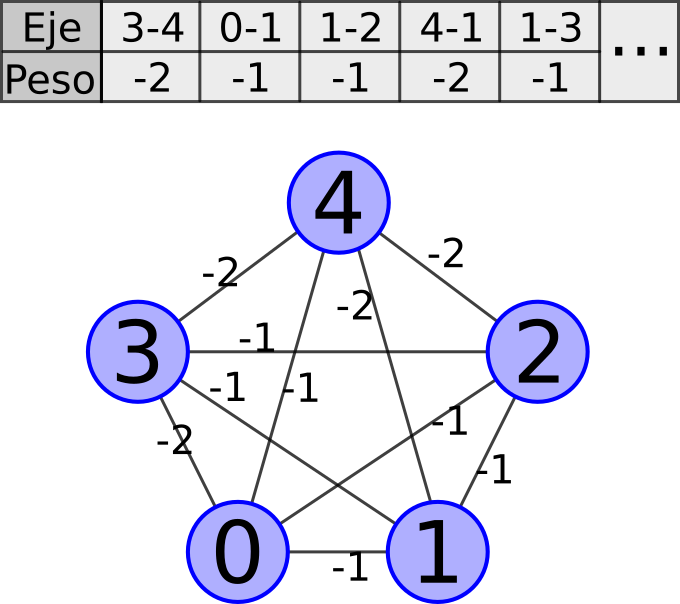
\includegraphics[width=4cm]{images/ej3/bestcase/00.png}} &
        \subfloat{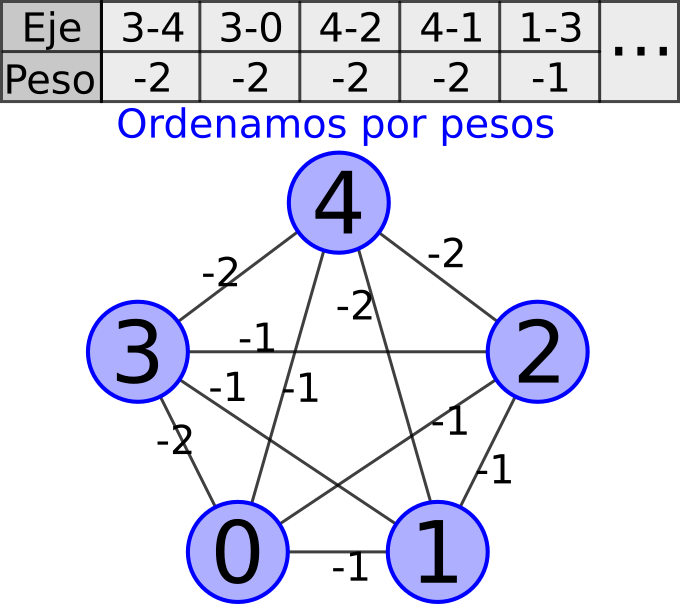
\includegraphics[width=4cm]{images/ej3/bestcase/01-sort.png}} &
        \subfloat{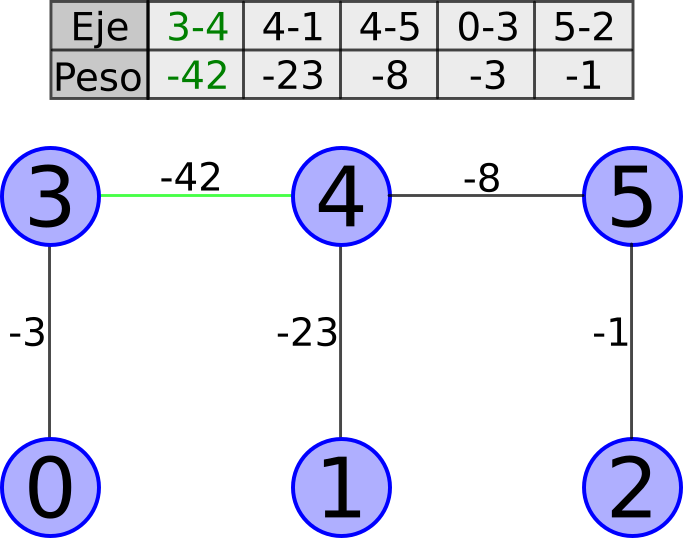
\includegraphics[width=4cm]{images/ej3/bestcase/02.png}} \\
        \subfloat{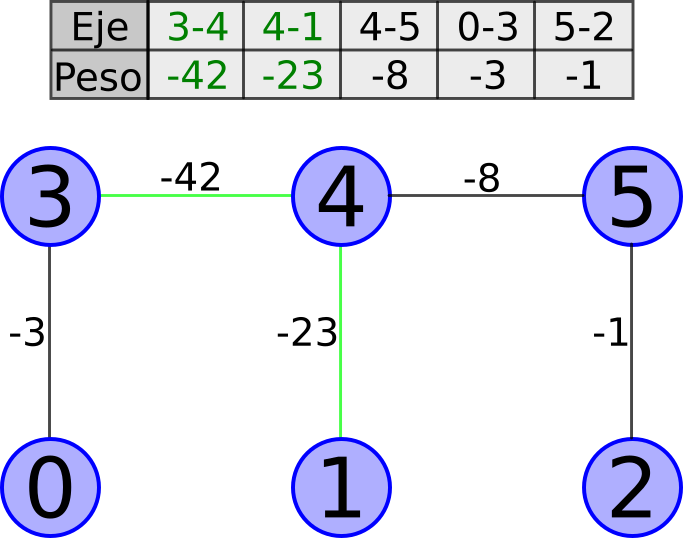
\includegraphics[width=4cm]{images/ej3/bestcase/03.png}} &
        \subfloat{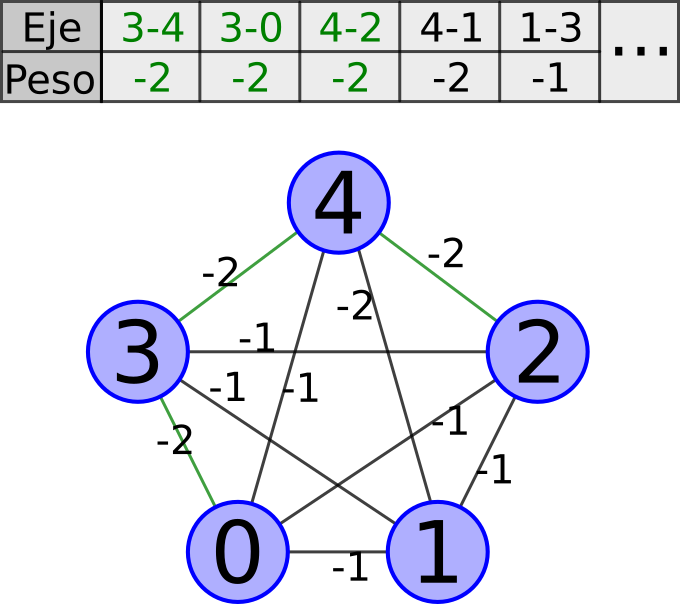
\includegraphics[width=4cm]{images/ej3/bestcase/04.png}} &
        \subfloat{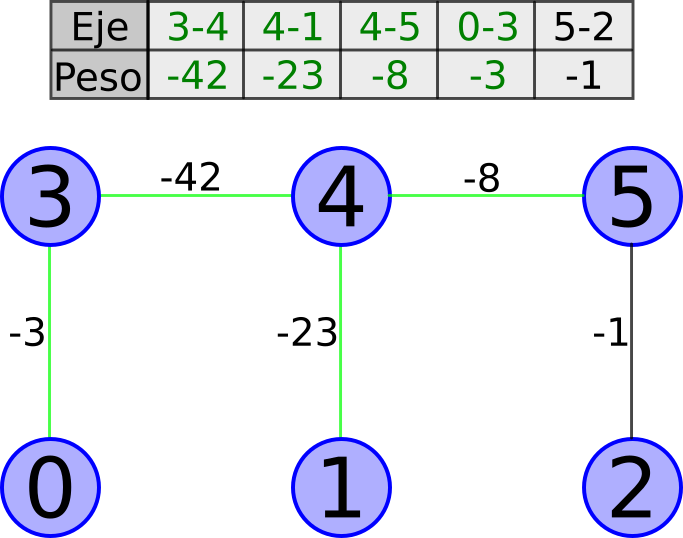
\includegraphics[width=4cm]{images/ej3/bestcase/05.png}} \\
        \subfloat{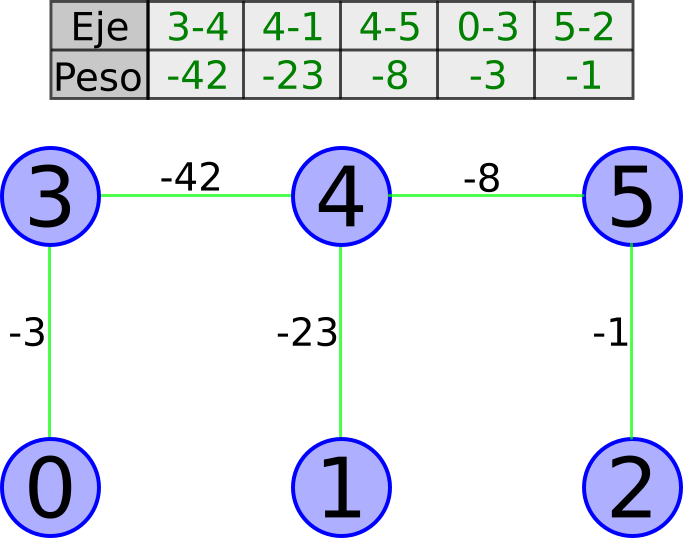
\includegraphics[width=4cm]{images/ej3/bestcase/06.png}} &
        \subfloat{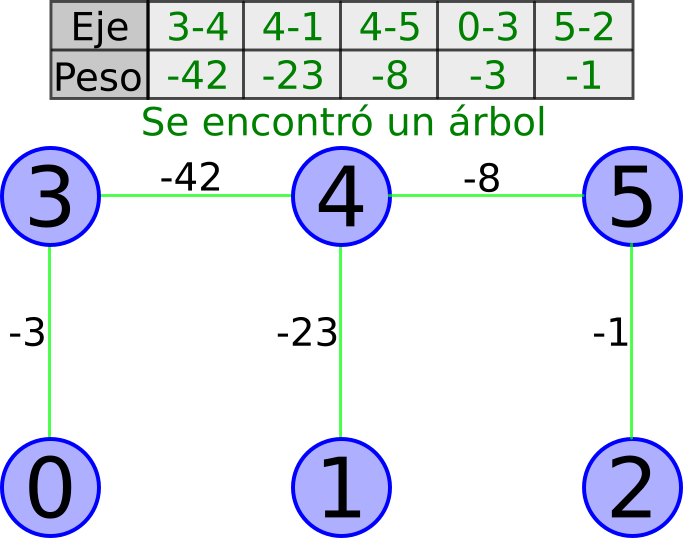
\includegraphics[width=4cm]{images/ej3/bestcase/07.png}}
    \end{tabular}
    
    \caption{Ejemplo de una corrida de mejor caso para el ejercicio 3. El arreglo de arriba representa el el vector interno de la cola de prioridad. \label{grf:ex3-best}}
\end{figure}

\pagebreak

Observemos que la transformación de los pesos de las aristas siempre toma exactamente $\Theta(m)$, ya que no nos queda otra más que recorrer todas las aristas para cambiar los pesos. Observemos, además, que en el algoritmo de Kruskal el mejor caso es en el que sólo tenemos que hacer heapify y tomar exactamente $n - 1$ aristas para completar el grafo sin encontrarnos ciclos, permitiéndonos entrar siempre dentro del if. Queda claro que esto sólo sucedería si el grafo fuese acíclico y tuviese exactamente $n - 1$ aristas, es decir, fuese un árbol. En este caso, tendríamos que $m \in O(n)$, y por lo tanto la complejidad temporal sería de $O(n log(n))$. Alternativamente, también podríamos pensar en un árbol generado como mencionamos anteriormente, pero agregarle aristas de peso menor a las que ya teníamos hasta completar el grafo: en este caso, la elección de aristas se verá forzada a concluir en exactamente $n - 1$ pasos, ya que las primeras $n - 1$ aristas del heap lograrán formar un árbol de peso máximo. \\

Por otro lado, caracterizar el peor caso es más difícil: si bien es claro que el grafo debería ser denso (teniendo entonces que ya el pre-procesamiento tomaría $\Theta(n^2)$), lo ideal sería también forzar al algoritmo de Kruskal a tener que hacer pop para todas las aristas antes de poder terminar. Observemos que el algoritmo va a hacer pop hasta que haya logrado completar un árbol, por lo que la condición fundamental para que esto suceda es que las aristas que le permitan completar un árbol sean las últimas en ser procesadas. Cabe destacar entonces que el pre-procesamiento lo que hace es dar vuelta el orden de recorrido de las aristas, por lo que las aristas que fuesen las primeras al ordenarlas en el grafo original van a ser las últimas en el grafo procesado; implicando que las aristas que para completar el árbol deberían ser las de menor peso del grafo. Finalmente, para generar un grafo de $n$ nodos con estas características lo único que debemos hacer es tomar $K_n$, asignar los pesos de cualquier forma (pero siempre mayores o iguales a un número $K > 1$), y luego tomar algún nodo arbitrario del grafo, y hacer que todas sus aristas tengan peso $K - 1$. Nótese, sin embargo, que jamás será posible popear exactamente todas las aristas, ya que al llegar a la primera de las que conectan al nodo, simplemente tomaremos a esa (y no va a haber una asignación de pesos particular que logre que esto cambie). En este caso, tendríamos que $m \in O(n^2)$, por lo que la complejidad temporal pasaría a ser $O(n^2 log(n))$.

\begin{figure}
    \centering
    
    \begin{tabular}{ccc}
        \subfloat{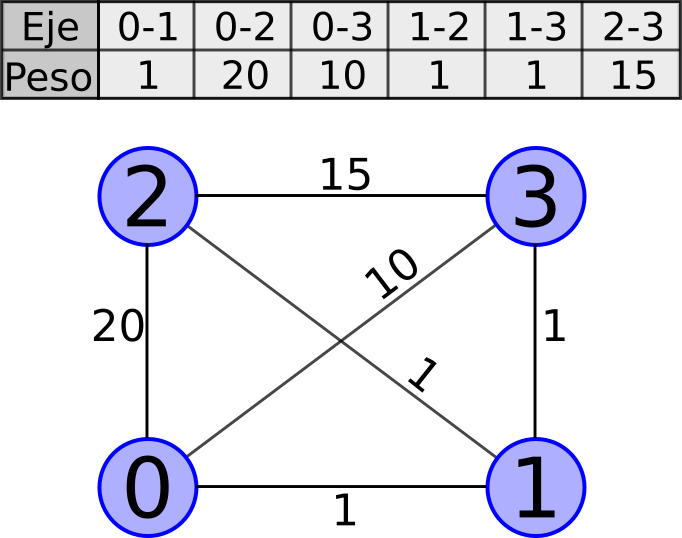
\includegraphics[width=4cm]{images/ej3/worstcase/00.png}} &
        \subfloat{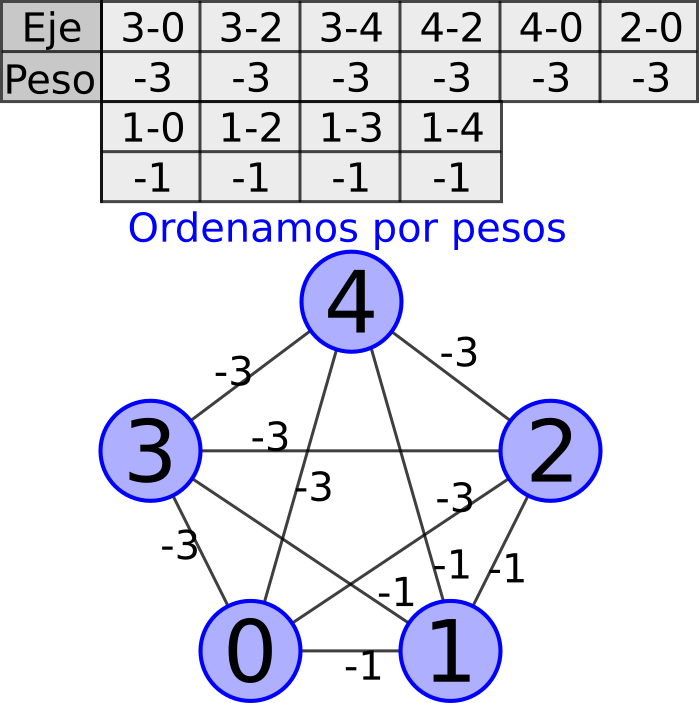
\includegraphics[width=4cm]{images/ej3/worstcase/01-sort.png}} &
        \subfloat{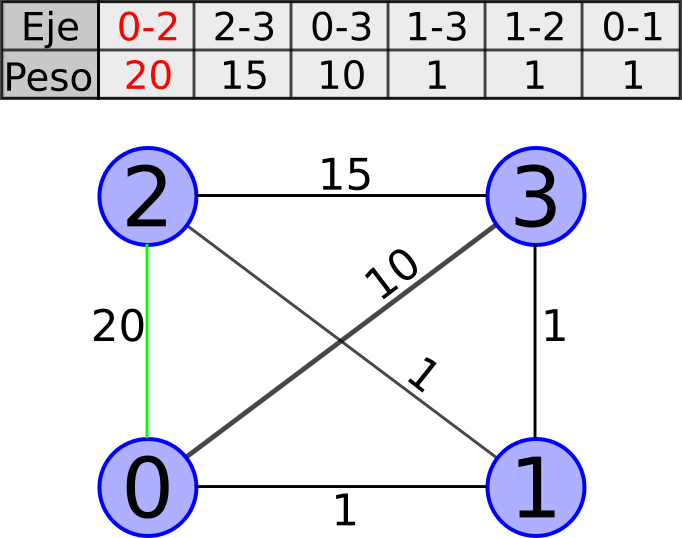
\includegraphics[width=4cm]{images/ej3/worstcase/02.png}} \\
        \subfloat{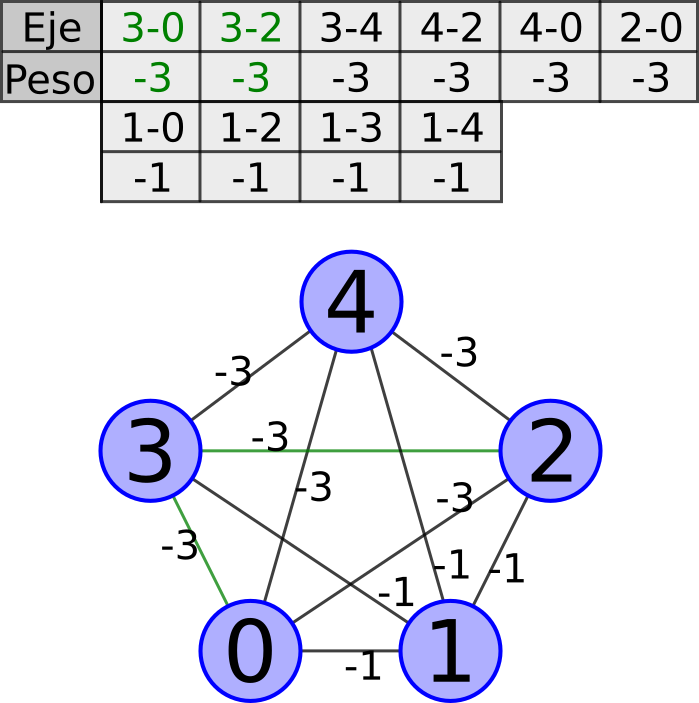
\includegraphics[width=4cm]{images/ej3/worstcase/03.png}} &
        \subfloat{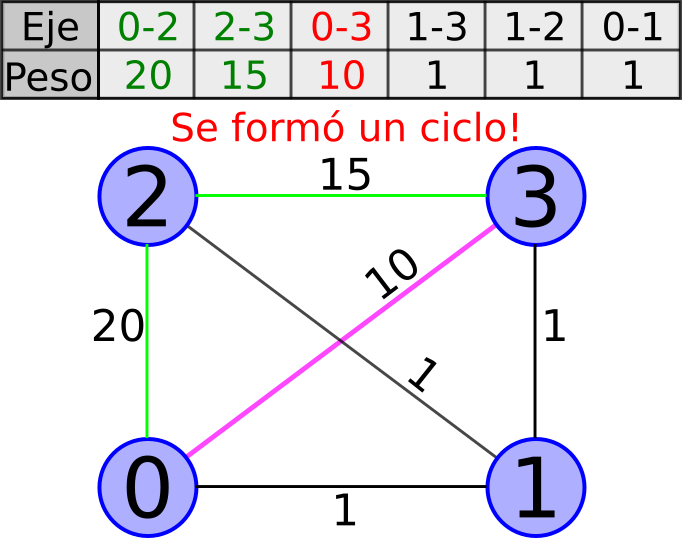
\includegraphics[width=4cm]{images/ej3/worstcase/04.png}} &
        \subfloat{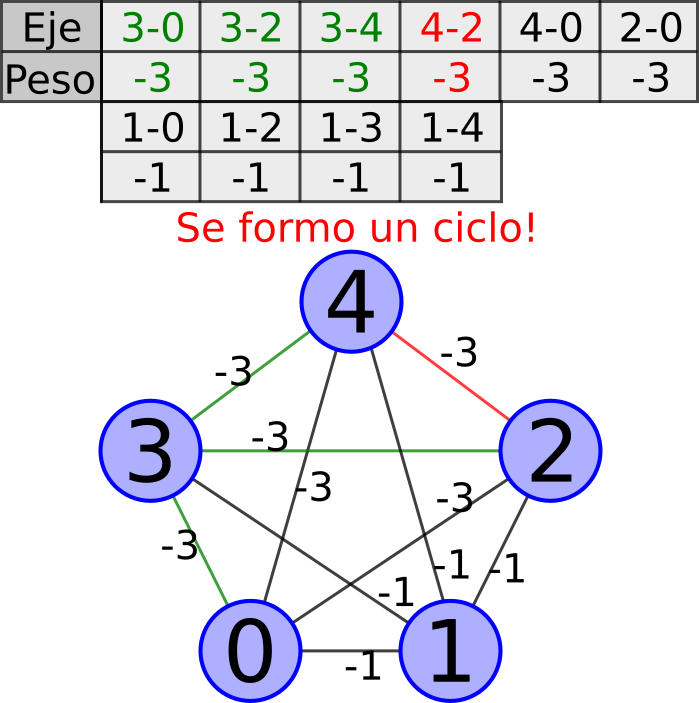
\includegraphics[width=4cm]{images/ej3/worstcase/05.png}} \\
        \subfloat{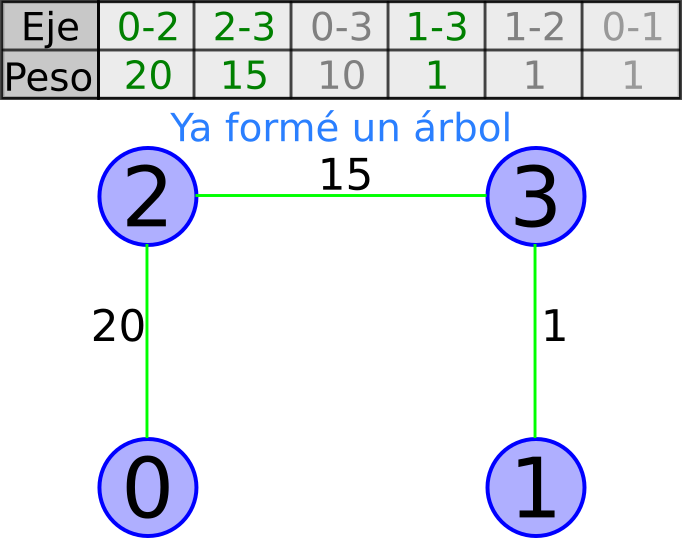
\includegraphics[width=4cm]{images/ej3/worstcase/06.png}}
    \end{tabular}
    
    \caption{Ejemplo de una corrida de peor caso para el ejercicio 3. El arreglo de arriba representa el el vector interno de la cola de prioridad. \label{grf:ex3-worst}}
\end{figure}

Como puede verse en la figura \ref{grf:ex3}, tenemos que ambos casos parecerían efectivamente estar en la complejidad deseada. Al igual que en los otros ejercicios, tenemos una variación muy amplia en la medición de tiempos al principio, pero terminan convergiendo a una constante, lo que demuestra que efectivamente la complejidad es como anunciamos anteriormente.

Para generar el mejor caso para este ejercicio, y que el $m$ sea el mismo para cada prueba que el $m$ en el peor caso, lo que hacemos es calcular a cada paso el $m$ correspondiente al peor caso, es decir, a un $K_n$ para un determinado $n$. Luego, generamos un árbol binario balanceado de $n$ nodos, donde cada arista tiene peso 2. Una vez hecho esto, se le agregan al árbol aristas aleatorias con peso 1 hasta que queda un grafo completo. De esta manera, cuando kruskal ordene las aristas, y saque las primeras $n-1$, ya va a tener el árbol armado y puede terminar, por lo que no hace falta que saque las $(n-1)*(n-2)/2$ aristas restantes.

Para generar los casos aleatorios para este ejercicio, como M en el peor caso es igual a $\frac{N*(N-1)}{2}$ ya que el peor caso es un $K_n$, lo que decidimos hacer es para cada N, generar
$K_n+1$, y elegir aleatoriamente $M+1$ aristas, siendo $M = \frac{N*(N-1)}{2}$. De esta manera, nos aseguramos que el grafo generado sea conexo, ya que si un grafo tiene $ M > \frac{(N-1)*(N-2)}{2}$ aristas, el mismo es conexo. Esto se debe a que $\frac{(N-1)*(N-2)}{2}$ es la cantidad de aristas de $K_n-1$, por lo que si agregamos un nodo más, y una arista más, por teorema del palomar, esa arista debe conectar a $K_n-1$ con el nuevo nodo, ya que $K_n-1$ es completo. La elección aleatoria de aristas da por resultado un grafo aleatorio, con la misma cantidad de aristas que el peor caso, ya que $O(M+1) = O(M)$.



\begin{figure}
\centering
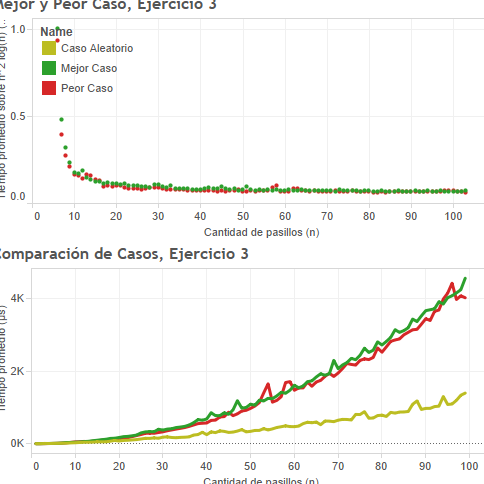
\includegraphics[width=10cm]{ex3}
\caption{El estadístico que tomamos es la media alfa podada de 100 corridas con $\alpha = 0.10$, que nos permite evitar algunos outliers. En ambos casos estamos graficando a las funciones sobre las complejidades esperadas. \label{grf:ex3}}
\end{figure}

\pagebreak

\section{Código fuente}

\lstset{inputencoding=utf8/latin1}
\lstset{basicstyle=\footnotesize\ttfamily,breaklines=true}
\lstset{framextopmargin=50pt,frame=bottomline}

\subsection{Main}
\lstinputlisting[language=C++]{../src/main.cpp}

\subsection{Ejercicio 1}
\lstinputlisting[language=C++]{../src/Exercise1.h}
\lstinputlisting[language=C++]{../src/Exercise1.cpp}

\subsection{Ejercicio 2}
\lstinputlisting[language=C++]{../src/Exercise2.h}
\lstinputlisting[language=C++]{../src/Exercise2.cpp}

\subsection{Ejercicio 3}
\lstinputlisting[language=C++]{../src/Exercise3.h}
\lstinputlisting[language=C++]{../src/Exercise3.cpp}

\end{document}